\documentclass{beamer}

\title{Modelos Generativos Profundos}
\subtitle{Clase 1: Introducción}
\author{Fernando Fêtis Riquelme}
\institute{
    Facultad de Ciencias Físicas y Matemáticas\\
    Universidad de Chile
}
\date{Primavera, 2025}
\titlegraphic{\hfill
\includegraphics[height=1.2cm]{fcfm}}

\usetheme{metropolis}
\setbeamercovered{transparent}

\begin{document}

\begin{frame}
    \titlepage
\end{frame}

\begin{frame}{Clase de hoy}
    \tableofcontents
\end{frame}

\section{Introducción a los modelos generativos modernos}

\begin{frame}{Qué son los modelos generativos y cómo funcionan}
    \begin{itemize}
        \item<1> Qué es un modelo generativo.
        \item<2> Aprendizaje supervisado vs. no supervisado.
        \item<3> Criterios de aprendizaje.
        \item<4> Generación condicional.
    \end{itemize}
\end{frame}

\begin{frame}{Qué puede generar un modelo generativo}
    Se pueden realizar múltiples tareas usando modelos generativos.
    \begin{itemize}
        \item<2> Creación y modificación de imágenes.
        \item<3> Generación de sonido y video.
        \item<4> Simular juegos.
        \item<5> LLMs en robótica.
        \item<6> Predicción de estructuras moleculares.
        \item<7> Otros estudios científicos.
    \end{itemize}
\end{frame}

\begin{frame}{Perspectivas para estudiar modelos generativos}
    Los modelos generativos actuales pueden ser estudiados desde distintos ángulos.
    \begin{itemize}
        \item<2> Perspectiva económica y social.
        \item<3> Perspectiva ética.
        \item<4> Interés filosófico.
        \item<5> Interés teórico.
    \end{itemize}
\end{frame}

\begin{frame}{Qué se estudiará en este curso}
    Los contenidos del curso son los siguientes.
    \begin{enumerate}
        \item<2> Introducción y repaso (1 semana).
        \item<3> Redes bayesianas (1 semana).
        \item<4> Modelos autorregresivos (3 semanas).
        \item<5> Redes generativas adversarias (2 semanas).
        \item<6> Autoencoders variacionales (2 semanas).
        \item<7> Flujos normalizantes (1 semana).
        \item<8> Modelos basados en energía (1 semana).
        \item<9> Modelos de difusión (2 semanas).
        \item<10> Modelos a tiempo continuo (2 semanas).

    \end{enumerate}
\end{frame}

\section{Requisitos y evaluaciones del curso}

\begin{frame}{Requisitos del curso}
    Si bien el curso es autocontenido, se asumen algunos conocimientos previos.
    \begin{itemize}
        \item<2,4> \textbf{Probabilidades:} distribuciones clásicas, variables independientes, probabilidad condicional, regla de Bayes, marginalización, verosimilitud, esperanza, etc.
        \item<3,4> \textbf{PyTorch:} creación de datasets, redes fully-connected, redes convolucionales, entrenamiento de modelos, etc.
    \end{itemize}
    \uncover<4>{Se realizará un repaso breve de estos temas en la siguiente clase.}
\end{frame}

\begin{frame}{Evaluaciones}
    Hay dos tipos de evaluación en el curso.
    \begin{itemize}
        \item<2,4> \textbf{Tareas (60\%):} (3 en total).
        \item<3,4> \textbf{Controles de lectura (40\%):} en horario de clases.
    \end{itemize}
    \uncover<4>{Ambos items deben ser aprobados por separado para aprobar el curso.}
\end{frame}

\begin{frame}{Evaluaciones}
    Algunas consideraciones.
    \begin{itemize}
        \item<2> Las tareas se realizan de forma individual.
        \item<3> Cada tarea tiene 2 semanas de plazo. \textbf{No se dará plazo adicional}.
        \item<4> De los 7 controles de lectura, se eliminan 2 para el cálculo de la nota.
        \item<5> Se pueden usar herramientas tipo ChatGPT para las tareas.
    \end{itemize}
\end{frame}

\section{Calendario y bibliografía}

\begin{frame}{Libros de referencia}
    Hay 3 libros que se recomiendan para el curso. El 1º sirve como introducción a cada tema, el 2º contiene la formalidad matemática, y el 3º contiene implementaciones en PyTorch.
    \vspace{0.3cm}
    \begin{center}
        \href{https://www.oreilly.com/library/view/generative-deep-learning/9781098134174/}{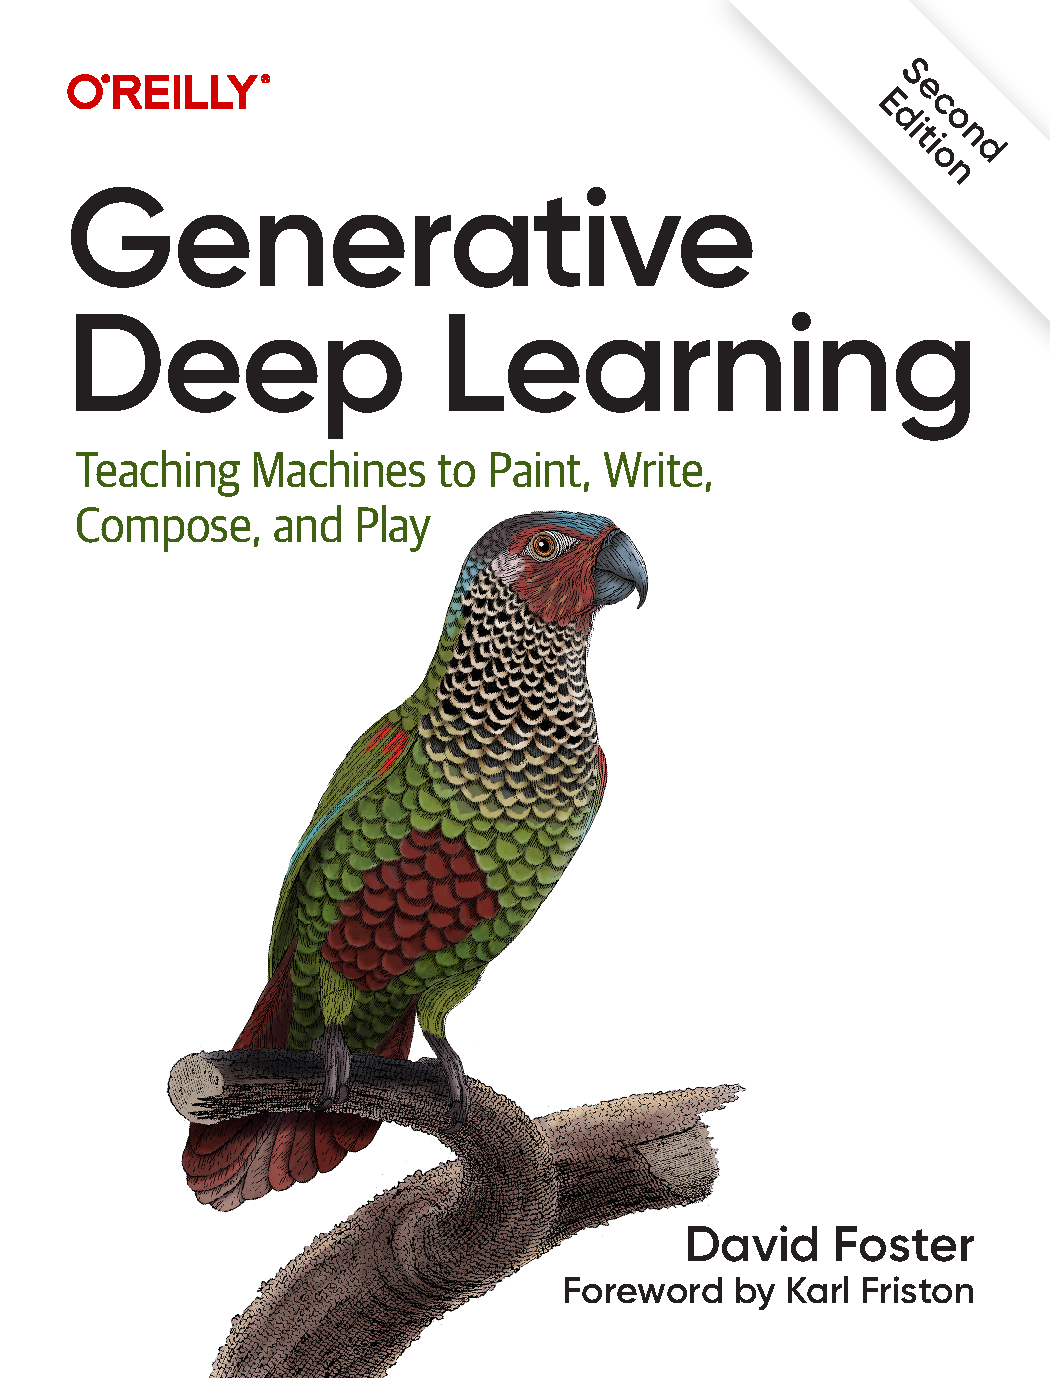
\includegraphics[width=0.3\textwidth]{foster.pdf}}
        \href{https://probml.github.io/pml-book/book2.html}{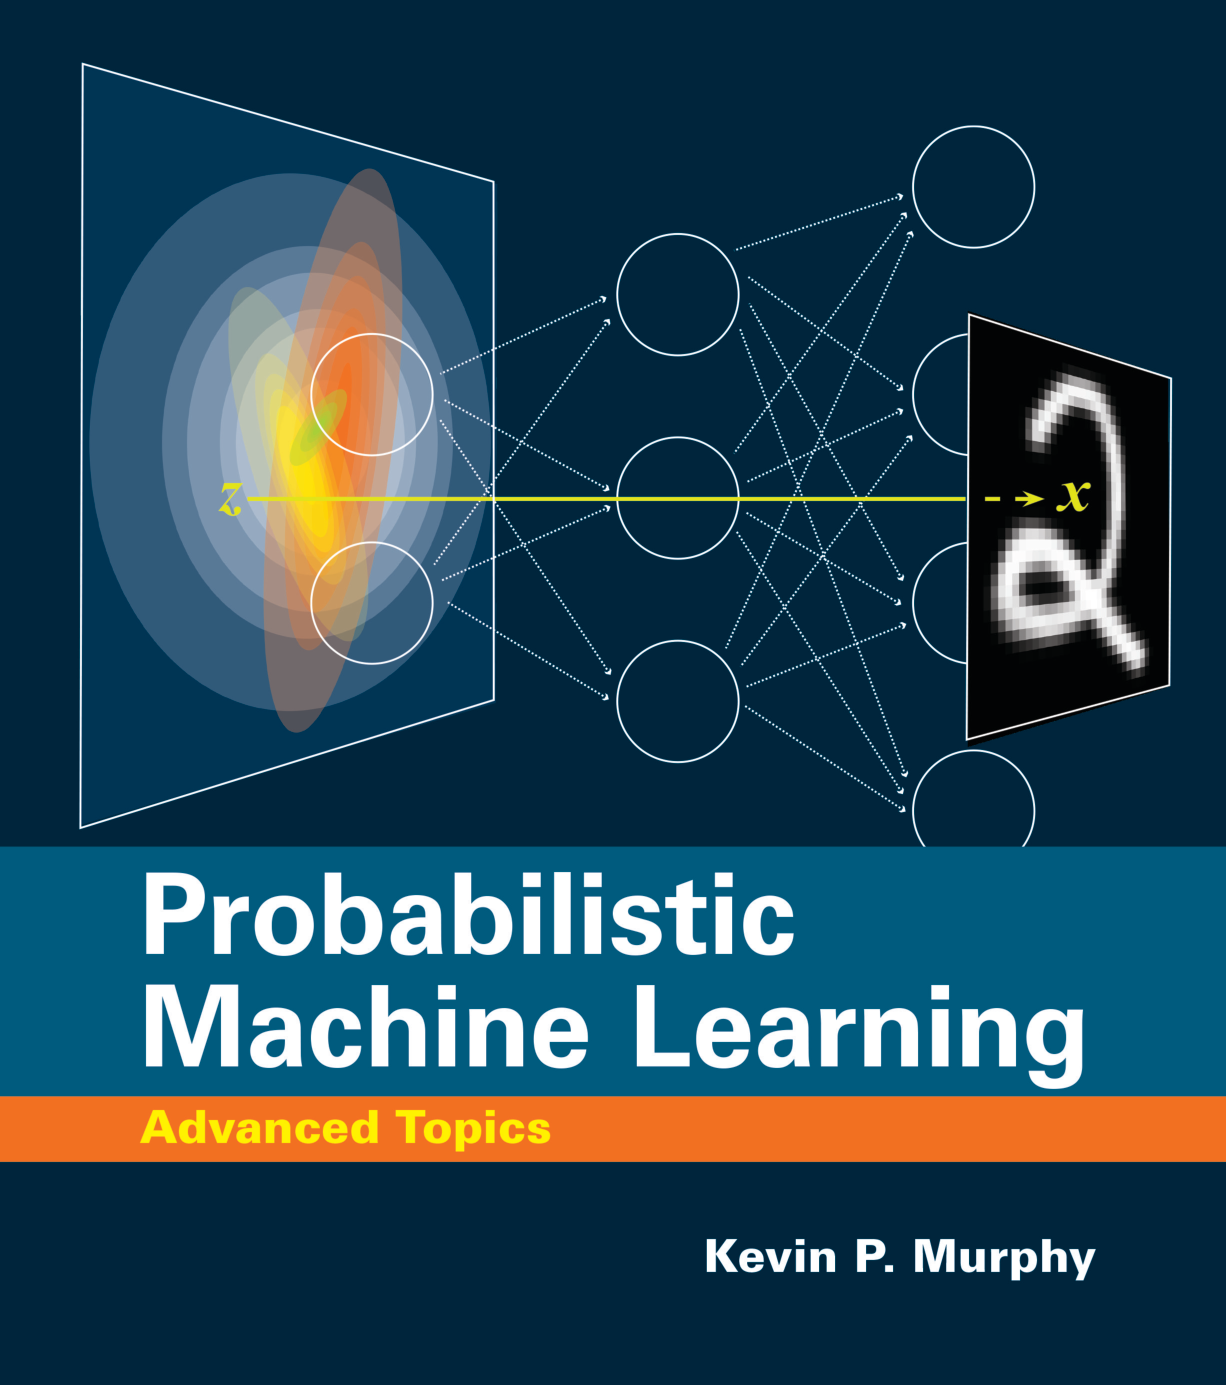
\includegraphics[width=0.3\textwidth]{murphy.pdf}}
        \href{https://link.springer.com/book/10.1007/978-3-031-64087-2}{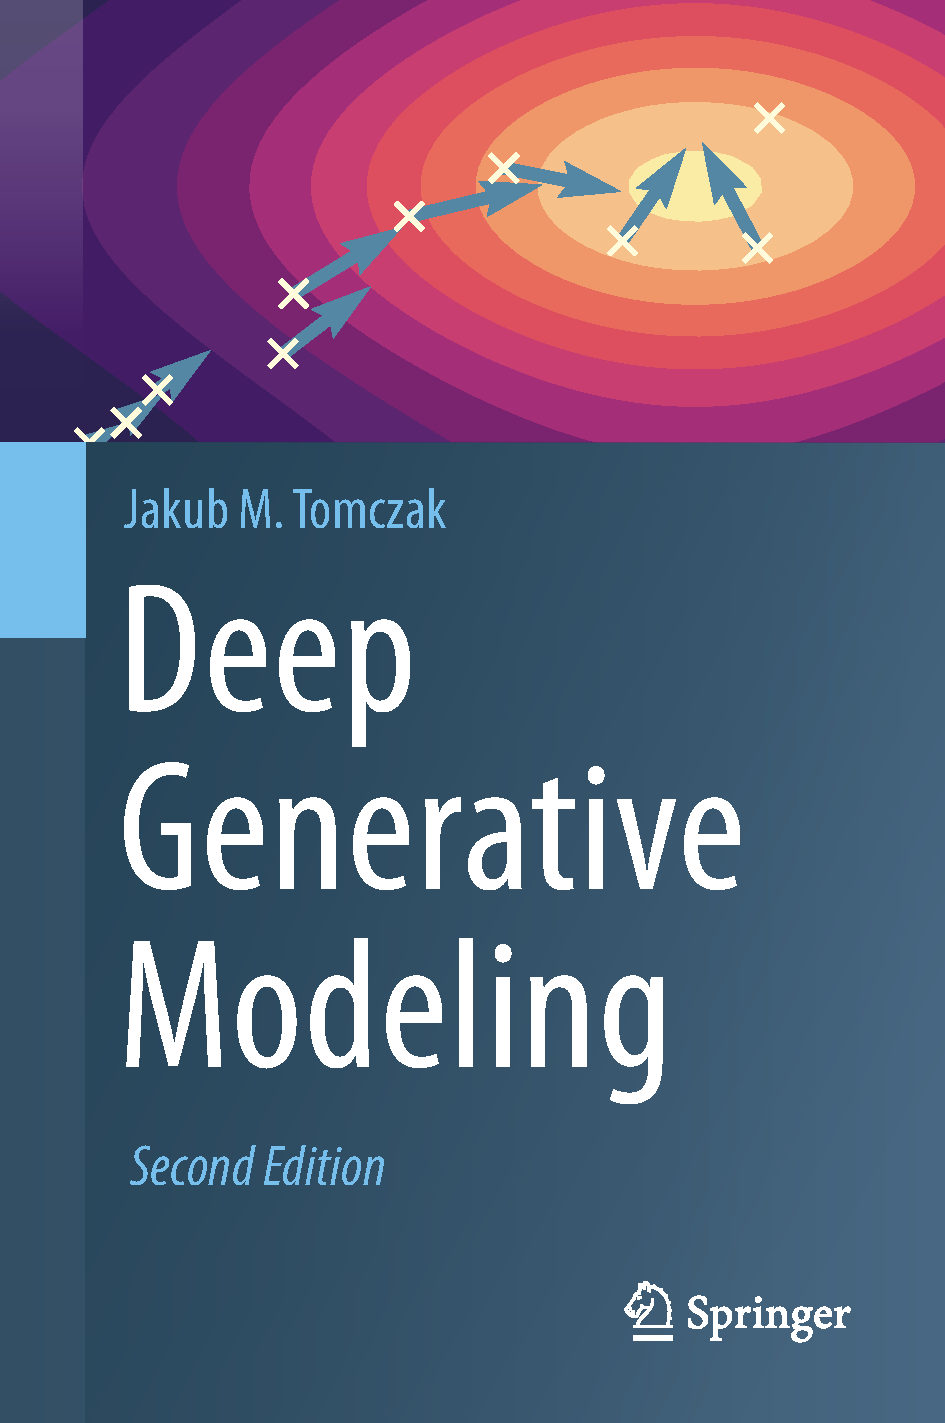
\includegraphics[width=0.3\textwidth]{tomczak.pdf}}
    \end{center}
\end{frame}

\begin{frame}{Próxima clase}
    En la próxima clase.
    \begin{itemize}
        \item<2> Se hará un repaso de conceptos de probabilidad y de PyTorch necesarios para el curso.
        \item<3> Se introducirán las redes bayesianas.
    \end{itemize}
\end{frame}

\begin{frame}
    \centering
    \Large{Modelos Generativos Profundos}\\
    \large{Clase 1: Introducción}
\end{frame}

\end{document}